\begin{frame}{Matrix Memory Preallocation}
\begin{itemize}
  \item PETSc sparse matrices are dynamic data structures
  \begin{itemize}
    \item can add additional nonzeros freely
  \end{itemize}

  \item Dynamically adding many nonzeros 
  \begin{itemize}
    \item requires additional memory allocations
    \item requires copies
    \item can kill performance
  \end{itemize}

  \item Memory preallocation provides
  \begin{itemize}
    \item the freedom of dynamic data structures
    \item good performance
  \end{itemize}

  \item Easiest solution is to replicate the assembly code
  \begin{itemize}
    \item Remove computation, but preserve the indexing code
    \item Store set of columns for each row
  \end{itemize}

  \item Call preallocation routines for all datatypes
  \begin{itemize}
    \item {\kb MatSeqAIJSetPreallocation()}
    \item {\kb MatMPIBAIJSetPreallocation()}
    \item Only the relevant data will be used
  \end{itemize}
\end{itemize}
\end{frame}

\begin{frame}{Sequential Sparse Matrices}
{\kb MatSeqAIJSetPreallocation(Mat A, int nz, int nnz[])}
\hbox{\qquad
\vbox{
\begin{itemize}
  \item[nz:] expected number of nonzeros in any row
  \item[nnz(i):] expected number of nonzeros in row i
\end{itemize}
}
}

\begin{center}
%\includegraphics[width=2in]{figures/Mat/serialSparseMatrix_bcsstk32}
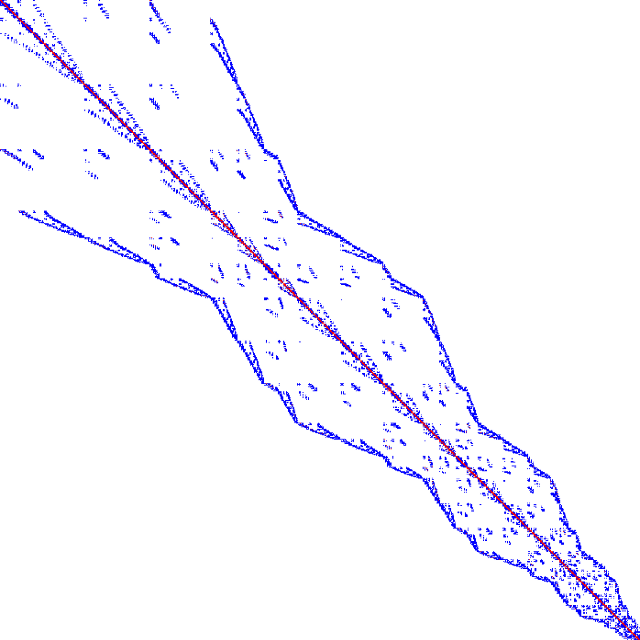
\includegraphics[width=.5\textwidth]{figures/EllipRCMSquare}
\end{center}
\end{frame}

\begin{frame}{Parallel Sparse Matrix}
\begin{itemize}
  \item Each process locally owns a submatrix of contiguous global rows
  \item Each submatrix consists of diagonal and off-diagonal parts
\end{itemize}

\begin{center}
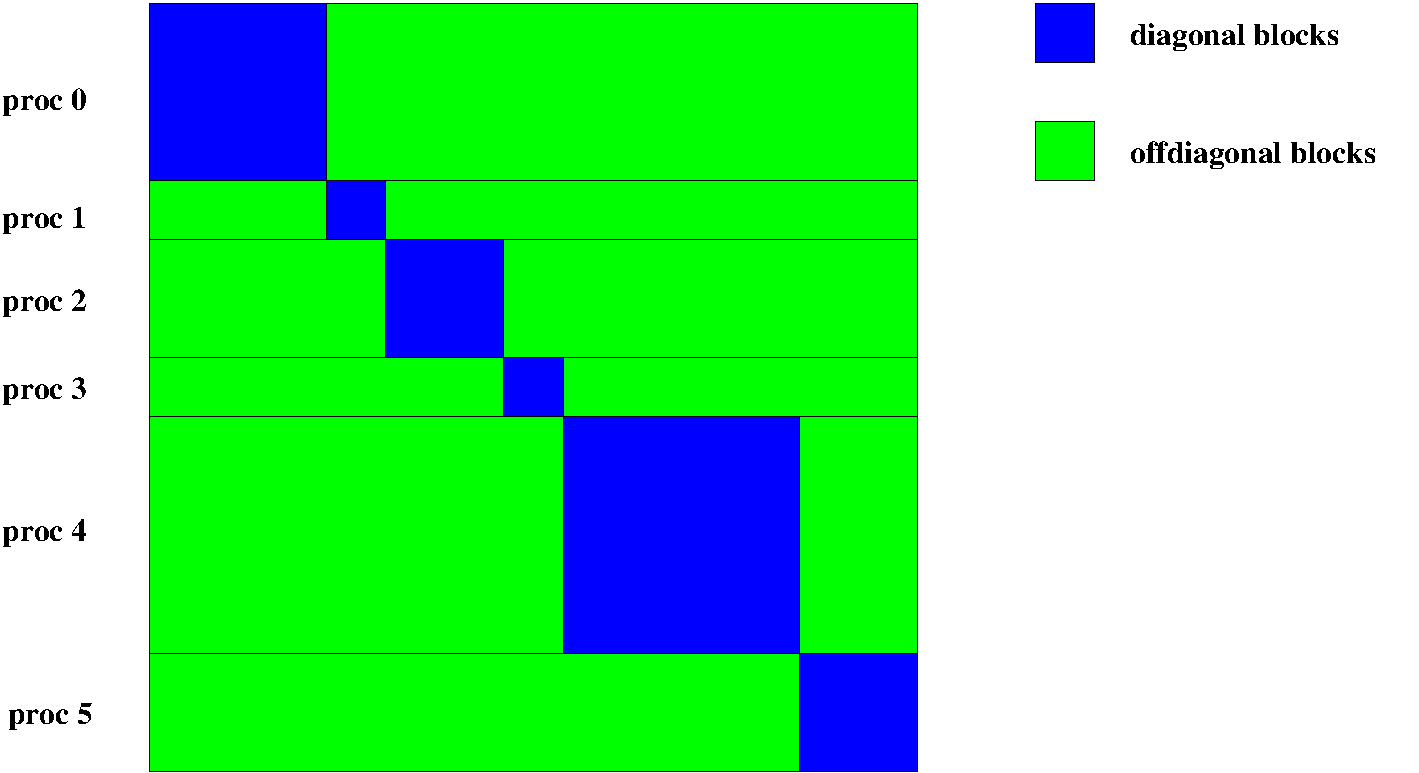
\includegraphics[width=3.5in]{figures/Mat/parallelSparseMatrix}
\end{center}

\begin{itemize}
  \item {\kb MatGetOwnershipRange(Mat A,int *start,int *end)}
  \begin{itemize}
    \item[{\kb start}:] first locally owned row of global matrix
    \item[{\kb end-1}:] last locally owned row of global matrix
  \end{itemize}
\end{itemize}
\end{frame}

\begin{frame}{Parallel Sparse Matrices}
\hbox{
\quad
\vbox{
{\kb MatMPIAIJSetPreallocation(Mat A, int dnz, int dnnz[], \\
  \qquad \qquad int onz, int onnz[])}
\begin{itemize}
  \item[dnz:] expected number of nonzeros in any row in the diagonal block
  \item[dnnz(i):] expected number of nonzeros in row i in the diagonal block
  \item[onz:] expected number of nonzeros in any row in the offdiagonal portion
  \item[onnz(i):] expected number of nonzeros in row i in the offdiagonal portion
\end{itemize}
}
}
\end{frame}

\begin{frame}{Verifying Preallocation}
\begin{itemize}
  \item Use runtime options \\
    {\kb -mat\_new\_nonzero\_location\_err} \\
    {\kb -mat\_new\_nonzero\_allocation\_err}
  \item Use runtime option {\kb -info}
  \item Output: \\
{\kb
  $[$proc \#$]$ Matrix size: \%d X \%d; storage space: \%d unneeded, \%d used \\
  $[$proc \#$]$ Number of mallocs during MatSetValues( )  is \%d
}
\end{itemize}

\bigskip

\begin{center}
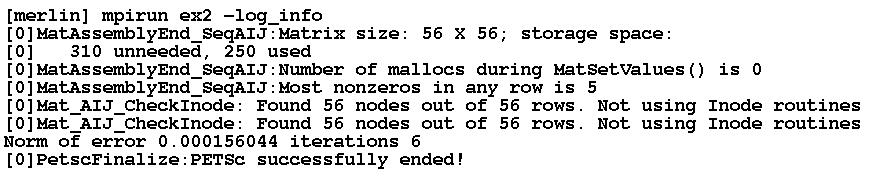
\includegraphics[width=5in]{figures/PETSc/logInfoOutput}
\end{center}
\end{frame}

\begin{frame}{Block and symmetric formats}
  \begin{itemize}
  \item BAIJ
    \begin{itemize}
    \item Like AIJ, but uses static block size
    \item Preallocation is like AIJ, but just one index per block
    \end{itemize}
  \item SBAIJ
    \begin{itemize}
    \item Only stores upper triangular part
    \item Preallocation needs number of nonzeros in upper triangular \\
      parts of on- and off-diagonal blocks
    \end{itemize}
  \item \code{MatSetValuesBlocked()}
    \begin{itemize}
    \item Better performance with blocked formats
    \item Also works with scalar formats, if \code{MatSetBlockSize()} was called
    \item Variants \code{MatSetValuesBlockedLocal()}, \code{MatSetValuesBlockedStencil()}
    \item Change matrix format at runtime, don't need to touch assembly code
    \end{itemize}
  \end{itemize}
\end{frame}
